%% LyX 2.3.6.1 created this file.  For more info, see http://www.lyx.org/.
%% Do not edit unless you really know what you are doing.
\documentclass[10pt,english,t,10pt,handout]{beamer}
\usepackage{lmodern}
\usepackage[T1]{fontenc}
\usepackage[utf8]{inputenc}
\setcounter{tocdepth}{1}
\setlength{\parskip}{\smallskipamount}
\setlength{\parindent}{0pt}
\usepackage{babel}
\usepackage{amsbsy}
\usepackage{amstext}
\usepackage{amssymb}
\usepackage{graphicx}
\usepackage[authoryear]{natbib}
\ifx\hypersetup\undefined
\AtBeginDocument{%
\hypersetup{unicode=true}
}
\else
\hypersetup{unicode=true}
\fi
\makeatletter
%%%%%%%%%%%%%%%%%%%%%%%%%%%%%% LyX specific LaTeX commands.
%% Because html converters don't know tabularnewline
\providecommand{\tabularnewline}{\\}
%%%%%%%%%%%%%%%%%%%%%%%%%%%%%% Textclass specific LaTeX commands.
% this default might be overridden by plain title style
\newcommand\makebeamertitle{\frame{\maketitle}}%
% (ERT) argument for the TOC
\AtBeginDocument{%
\let\origtableofcontents=\tableofcontents
\def\tableofcontents{\@ifnextchar[{\origtableofcontents}{\gobbletableofcontents}}
\def\gobbletableofcontents#1{\origtableofcontents}
}
%%%%%%%%%%%%%%%%%%%%%%%%%%%%%% User specified LaTeX commands.
\usepackage{tikz}
\usetikzlibrary{positioning}
\usepackage{appendixnumberbeamer}
\usepackage{graphicx}
\usepackage{subfig}
\usetheme[progressbar=frametitle,block=fill,subsectionpage=progressbar]{metropolis}
% margin
\setbeamersize{text margin right=1.5cm}
% colors
\definecolor{DarkRed}{rgb}{0.7,0,0}
%\colorlet{DarkRed}{redblack}
\setbeamercolor{normal text}{fg=black}
\setbeamercolor{alerted text}{fg=DarkRed}
\setbeamercolor{progress bar}{fg=DarkRed}
\setbeamercolor{button}{bg=DarkRed}
% width of seperators
\makeatletter
\setlength{\metropolis@titleseparator@linewidth}{1pt}
\setlength{\metropolis@progressonsectionpage@linewidth}{1pt}
\setlength{\metropolis@progressinheadfoot@linewidth}{1pt}
\makeatother
% new alert block
\newlength\origleftmargini
\setlength\origleftmargini\leftmargini
\setbeamertemplate{itemize/enumerate body begin}{\setlength{\leftmargini}{4mm}}
\let\oldalertblock\alertblock
\let\oldendalertblock\endalertblock
\def\alertblock{\begingroup \setbeamertemplate{itemize/enumerate body begin}{\setlength{\leftmargini}{\origleftmargini}} \oldalertblock}
\def\endalertblock{\oldendalertblock \endgroup}
\setbeamertemplate{mini frame}{}
\setbeamertemplate{mini frame in current section}{}
\setbeamertemplate{mini frame in current subsection}{}
\setbeamercolor{section in head/foot}{fg=normal text.bg, bg=structure.fg}
\setbeamercolor{subsection in head/foot}{fg=normal text.bg, bg=structure.fg}
% footer
\makeatletter
\setbeamertemplate{footline}{%
\begin{beamercolorbox}[colsep=1.5pt]{upper separation line head}
\end{beamercolorbox}
\begin{beamercolorbox}{section in head/foot}
\vskip1pt\insertsectionnavigationhorizontal{\paperwidth}{}{\hskip0pt plus1filll \insertframenumber{} / \inserttotalframenumber \hskip2pt}\vskip3pt% 
\end{beamercolorbox}%
\begin{beamercolorbox}[colsep=1.5pt]{lower separation line head}
\end{beamercolorbox}
}
\makeatother
% toc
\setbeamertemplate{section in toc}{\hspace*{1em}\inserttocsectionnumber.~\inserttocsection\par}
\setbeamertemplate{subsection in toc}{\hspace*{2em}\inserttocsectionnumber.\inserttocsubsectionnumber.~\inserttocsubsection\par}
\makeatother
\begin{document}
\title{3. Stationary Equilibrium\vspace{-2mm}}
\subtitle{Adv. Macro: Heterogenous Agent Models} 
\author{Nicolai Waldstrøm}
\date{2024}
{
\setbeamertemplate{footline}{} 
\begin{frame}
\maketitle
\begin{tikzpicture}[overlay, remember picture]
\node[above left=-0.14cm and -0.14cm of current page.south east] 
{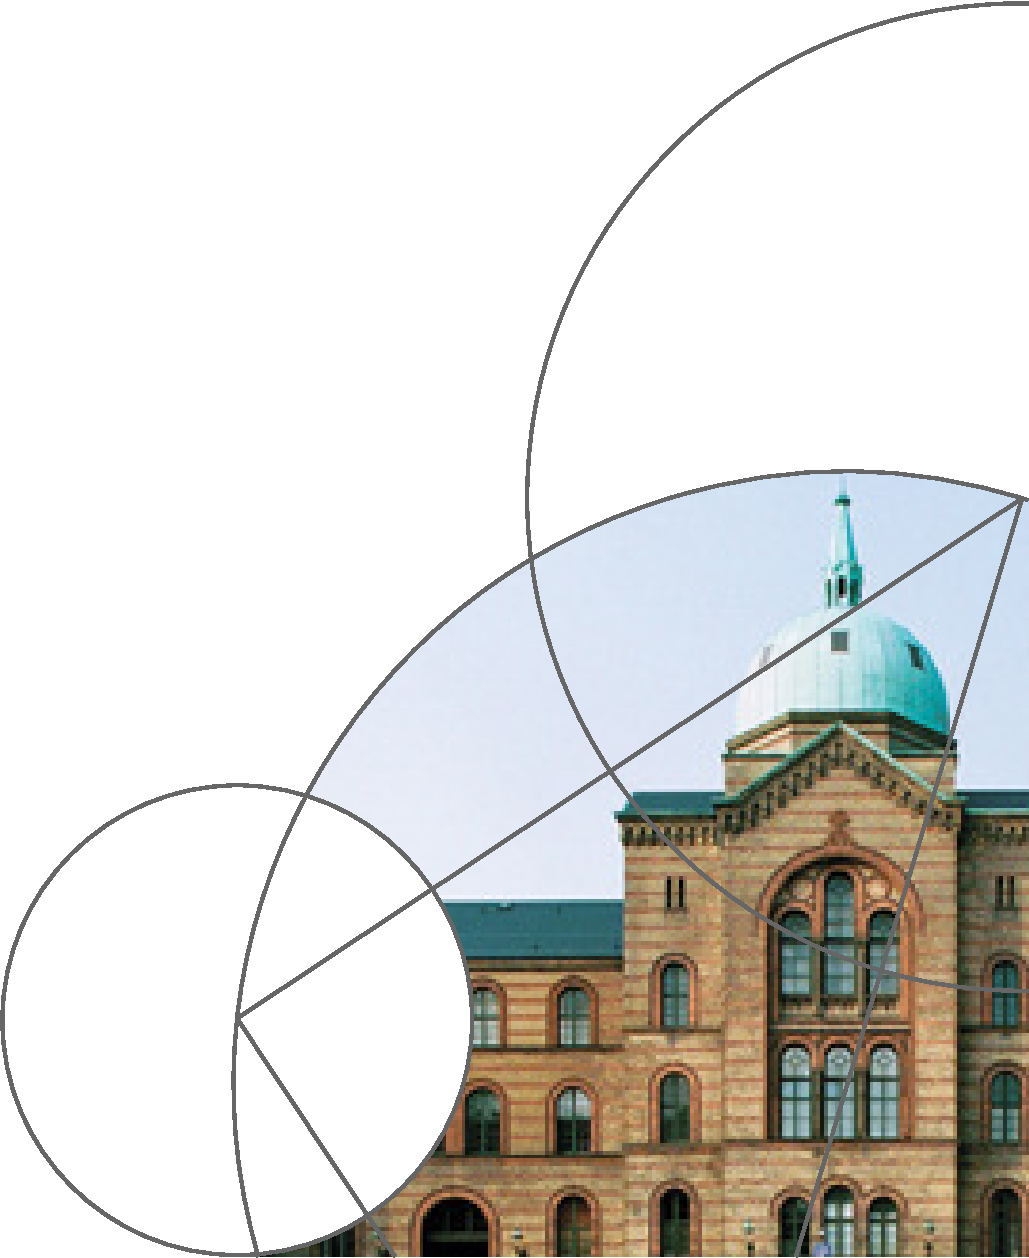
\includegraphics[width=4cm]{figs/KUSAMFtitlelrcorner.pdf}};
\end{tikzpicture}
\begin{tikzpicture}[overlay, remember picture]
\node[below left=0.5cm and .8cm of current page.north east] 
{\includegraphics[width=1.5cm]{figs/KUSAMFlogo.pdf}};
\end{tikzpicture}
\end{frame}
}
\addtocounter{framenumber}{-1}
\section{Introduction}
\begin{frame}{Introduction}
\vspace{-2mm}
\begin{itemize}
\item <+->\textbf{Last time: }
\begin{enumerate}
\item Partial equilibrium 
\item No interactions 
\end{enumerate}
\item <+->\textbf{Today:} Interaction through markets
\item <+->\textbf{Model:} Heterogeneous Agent Neo-Classical (HANC) model
\item <+->\textbf{Equilibrium-concept:} \emph{Stationary equilibrium}
\begin{enumerate}
\item What determines income and wealth inequality\emph{ in the long run}?
\item What determines the real interest rate \emph{in the long run}?
\end{enumerate}
\item <+->\textbf{Code:} Based on the \textcolor{DarkRed}{\href{https://github.com/NumEconCopenhagen/GEModelTools}{GEModelTools}}
package
\begin{enumerate}
\item Is in active development
\item You can help to improve interface, find bugs and features 
\end{enumerate}
\textbf{Documentation: }See \textcolor{DarkRed}{\href{https://github.com/NumEconCopenhagen/GEModelToolsNotebooks}{GEModelToolsNotebooks}}
\begin{itemize}
\item Many examples in repo, so look if you have issues 
\end{itemize}
\item <+->\textbf{Literature:} Aiyagari (1994) 
\end{itemize}
\end{frame}
%
\section{Ramsey-recap}
\begin{frame}{The Ramsey model}
\begin{itemize}
\item <+->We will study the \emph{stationary equilibrium }in\emph{ }the\emph{
}Heterogeneous Agent Neo-Classical (HANC) model
\item <+->Merges two well known models in the literature:
\begin{itemize}
\item <+->Standard Ramsey–Cass–Koopman model (\emph{NC})
\begin{itemize}
\item What do we mean by Neo-classical? 
\end{itemize}
\item <+->One-asset Buffer-stock model (\emph{HA})
\end{itemize}
\item <+->Went through the Buffer-stock model over the last two lectures 
\item <+->\textbf{Now}: Recap of the Ramsey model 
\end{itemize}
\end{frame}
%
\begin{frame}{Ramsey: Firms}
\begin{itemize}
\item <+->\textbf{Production function: $Y_{t}=F(\Gamma_{t},K_{t-1},L_{t})$
}{\footnotesize{}{[}note timing of capital{]}}{\footnotesize\par}
where $\Gamma_{t}$ is technology
\item <+->\textbf{Profits:} $\Pi_{t}=Y_{t}-w_{t}L_{t}-r_{t}^{K}K_{t-1}$ 
\item <+->\textbf{Profit maximization: $\max_{K_{t-1},L_{t}}\Pi_{t}$}\vspace{1mm}
\begin{enumerate}
\item Rental rate: $\frac{\partial\Pi_{t}}{\partial K_{t-1}}=0\Leftrightarrow$$r_{t}^{K}=F_{K}(\Gamma_{t},K_{t-1},L_{t})$\vspace{1mm}
\item Real wage: $\frac{\partial\Pi_{t}}{\partial L_{t}}=0\Leftrightarrow w_{t}=F_{L}(\Gamma_{t},K_{t-1},L_{t})$\vspace{1mm}
\end{enumerate}
\vspace{1mm}With CRS we get zero profits: $\Pi_{t}=0\Rightarrow$\vspace{2mm}
$Y_{t}=w_{t}L_{t}+r_{t}^{K}K_{t-1}$ {\footnotesize{}{[}functional
income distribution{]}}{\footnotesize\par}
\end{itemize}
\end{frame}
%
\begin{frame}{Ramsey: Zero-profit mutual fund}
\begin{itemize}
\item <+->Introduce \textbf{mutual fund}
\begin{itemize}
\item Takes savings $A_{t-1}$ from households and investment them in available
assets
\item In the Ramsey model: Only capital $K_{t-1}$ but could also include
gov. bonds, firm equity etc.
\end{itemize}
\item <+->\textbf{Capital depreciate }with rate $\delta\in(0,1)$,\textbf{
\[
K_{t}=(1-\delta)K_{t-1}+I_{t}
\]
}
\item <+->\textbf{Deposits }(from households), $A_{t-1}$:\textbf{ }The
rate of return is 
\[
r_{t}=r_{t}^{K}-\delta
\]
\item <+->\textbf{Balance sheet:
\[
A_{t-1}=K_{t-1}
\]
}
\end{itemize}
\end{frame}
%
\begin{frame}{Ramsey: Households}
\begin{itemize}
\item \textbf{Utility maximization:}\vspace{-2mm}
\begin{align*}
v_{0}(A_{-1}^{hh}) & =\max_{\{C_{t}^{hh}\}_{t=0}^{\infty}}\sum_{t=0}^{\infty}\beta^{t}u(C_{t}^{hh})\\
& \text{s.t.}\\
C_{t}^{hh}+A_{t}^{hh} & =(1+r_{t})A_{t-1}^{hh}+w_{t}L_{t}^{hh}
\end{align*}
Exogenous labor supply: $L_{t}^{hh}=1$
\item \textbf{Euler-equation }(implied by Lagrangian):\textbf{
\[
u^{\prime}(C_{t}^{hh})=\beta(1+r_{t+1})u^{\prime}(C_{t+1}^{hh})
\]
}
\end{itemize}
\end{frame}
%
\begin{frame}{Ramsey: Market Clearing}
\begin{itemize}
\item <+->\textbf{Capital market: $K_{t}=A_{t}=A_{t}^{hh}$}
\item <+->\textbf{Labor market: $L_{t}=L_{t}^{hh}=1$}
\item <+->\textbf{Goods market: $Y_{t}=C_{t}^{hh}+I_{t}$}\vspace{2mm}
\item <+->\textbf{Walras:} Capital and labor market clears $\Rightarrow$
goods market clears. Start from 
\begin{align*}
C_{t}^{hh}+A_{t}^{hh} & =(1+r_{t})A_{t-1}^{hh}+w_{t}L_{t}^{hh})\\
\Leftrightarrow C_{t}^{hh}+I_{t} & =\left[(1+r_{t})A_{t-1}^{hh}+w_{t}L_{t}^{hh}-A_{t}^{hh})\right]+(K_{t}-(1-\delta)K_{t-1})\\
& =\left[(1+r_{t})K_{t-1}+w_{t}L_{t}-K_{t})\right]+(K_{t}-(1-\delta)K_{t-1})\\
& =r_{t}^{K}K_{t-1}+w_{t}L_{t}\\
& =Y_{t}
\end{align*}
\item <+->Note: Means that we can check if we have solved the numerical
model correctly by: 
\begin{itemize}
\item Impose two of the market clearing conditions
\item Then check the third market clearing condition (should be zero)
\end{itemize}
\end{itemize}
\end{frame}
%
\begin{frame}{Ramsey: Summary}
\begin{itemize}
\item <+->\textbf{Simplified form:}
\begin{align*}
u^{\prime}(C_{t}^{hh}) & =\beta(1+F_{K}(\Gamma_{t},K_{t},1)-\delta)u^{\prime}(C_{t+1}^{hh})\\
K_{t} & =(1-\delta)K_{t-1}+F(\Gamma_{t},K_{t-1},1)-C_{t}^{hh}
\end{align*}
\item <+->\textbf{Extended form:}\vspace{-1mm}\textbf{
\begin{align*}
r_{t}^{K} & =F_{K}(\Gamma_{t},K_{t-1},L_{t})\\
w_{t} & =F_{L}(\Gamma_{t},K_{t-1},L_{t})\\
r_{t} & =r_{t}^{K}-\delta\\
A_{t} & =K_{t}\\
A_{t}^{hh} & =(1+r_{t})A_{t-1}^{hh}+w_{t}L_{t}^{hh}-C_{t}^{hh}\\
u^{\prime}(C_{t}^{hh}) & =\beta(1+r_{t+1})u^{\prime}(C_{t+1}^{hh})\\
A_{t} & =A_{t}^{hh}\\
L_{t} & =L_{t}^{hh}
\end{align*}
}
\end{itemize}
\end{frame}
%
\begin{frame}{Ramsey: As an equation system}
Eqs. system with unknowns $\left\{ K_{t},L_{t},r_{t}^{K},w_{t},r_{t},A_{t},A_{t}^{hh},C_{t}^{hh}\right\} _{t=0}^{\infty}$
and eqs:
\begin{align*}
\left[\begin{array}{c}
r_{t}^{K}-F_{K}(\Gamma_{t},K_{t-1},L_{t})\\
w_{t}-F_{L}(\Gamma_{t},K_{t-1},L_{t})\\
r_{t}-(r_{t}^{K}-\delta)\\
A_{t}-K_{t}\\
A_{t}^{hh}-\left((1+r_{t})A_{t-1}^{hh}+w_{t}L_{t}^{hh}-C_{t}^{hh}\right)\\
u^{\prime}(C_{t}^{hh})-\beta(1+r_{t+1})u^{\prime}(C_{t+1}^{hh})\\
A_{t}-A_{t}^{hh}\\
L_{t}-L_{t}^{hh}\\
\forall t\in\{0,1,\dots\},\text{given }K_{-1}
\end{array}\right] & \boldsymbol{=}\boldsymbol{0}
\end{align*}
\end{frame}
%
\begin{frame}{Ramsey: Steady state}
\begin{itemize}
\item \textbf{Euler-equation} can be solved for $K_{ss}$:
\begin{align*}
u^{\prime}(C_{ss}) & =\beta(1+F_{K}(\Gamma_{ss},K_{ss},1)-\delta)u^{\prime}(C_{ss})\Leftrightarrow\\
F_{K}(K_{ss},1) & =\frac{1}{\beta}-1+\delta
\end{align*}
\item \textbf{Accumulation equation + goods mkt. clearing} then implies
$C_{ss}$:
\begin{align*}
K_{ss} & =(1-\delta)K_{ss}+F(\Gamma_{ss},K_{ss},1)-C_{ss}\Leftrightarrow\\
C_{ss} & =(1-\delta)K_{ss}+F(\Gamma_{ss},K_{ss},1)-K_{ss}
\end{align*}
\end{itemize}
\end{frame}
%
\section{HANC}
\begin{frame}{HANC model overview}
\begin{itemize}
\item <+->\textbf{Model blocks:}
\begin{enumerate}
\item \textbf{Firms:} Rent capital from mutual fund and hire labor from
the households, produce with given technology, and sell output goods
\item \textbf{Zero-profit mutual funds:} Own capital and rent it to firms,
take deposits and pay return to household
\item \textbf{Households:} Face idiosyncratic productivity shocks, supplies
labor exogenously and makes consumption-saving decisions
\item \textbf{Markets:} Perfect competition in labor, goods and capital
markets
\end{enumerate}
\item <+->\textbf{Add-on to Ramsey-Cass-Koopman:} \emph{Heterogeneous households}
\item <+->\textbf{Other names:}
\begin{enumerate}
\item <+->The Aiyagari-model
\item <+->The Aiyagari-Bewley-Hugget-Imrohoroglu-model
\item <+->The Standard Incomplete Market (SIM) model
\end{enumerate}
\end{itemize}
\end{frame}
%
\begin{frame}{Heterogeneous households}
\begin{itemize}
\item <+->\textbf{Utility maximization} for household $i$:\vspace{-2mm}
\begin{align*}
v_{0}(\beta_{i},z_{it},a_{it-1}) & =\max_{\{c_{it}\}_{t=0}^{\infty}}\mathbb{E}_{0}\sum_{t=0}^{\infty}\beta_{i}^{t}u(c_{it})\\
& \text{s.t.}\\
\ell_{it} & =z_{it}\\
a_{it} & =(1+r_{t})a_{it-1}+w_{t}\ell_{it}-c_{it}+\Pi_{t}\\
\log z_{it+1} & =\rho_{z}\log z_{it}+\psi_{it+1},\,\,\,\psi_{it}\sim\mathcal{N}(\mu_{\psi},\sigma_{\psi}),\,\,\,\mathbb{E}[z_{it}]=1\\
a_{it} & \geq0
\end{align*}
\item <+->\vspace{-1mm}\textbf{Where does heterogeneity enter?}
\begin{enumerate}
\item <+-|handout:0>\emph{Ex ante} due to different preferences, $\beta_{i}$
\item <+-|handout:0>\emph{Ex post} due to stochastic productivity, $z_{it}$
\end{enumerate}
\item <+->\textbf{Incomplete markets due to borrowing constraint }\\
{\small{}(fancy words: partial self-insurrance, lack of Arrow-Debreu
securities)}{\small\par}
\end{itemize}
\end{frame}
%
\begin{frame}{Recursive formulation}
\begin{itemize}
\item <1->\textbf{Value function }(at decision)
\begin{align*}
v_{t}(\beta_{i},z_{it},a_{it-1}) & =\max_{c_{t}}u(c_{t})+\beta\underline{v}_{t+1}(\beta_{i},z_{it},a_{it})\\
& \text{s.t.}\\
\ell_{it} & =z_{it}\\
a_{it} & =(1+r_{t})a_{it-1}+w_{t}\ell_{it}-c_{it}+\Pi_{t}\\
\log z_{it+1} & =\rho_{z}\log z_{it}+\psi_{it+1}\\
a_{it} & \geq0
\end{align*}
\item <1->\textbf{Beginning-of-period value function} (before shock realization):
\[
\underline{v}_{t}(\beta_{i},z_{it-1},a_{it-1})=\mathbb{E}\left[v_{t}(\beta_{i},z_{it},a_{it-1})\,|\,\beta_{i},z_{it-1},a_{it-1}\right]
\]
\end{itemize}
\end{frame}
%
\begin{frame}{Distributions and aggregates}
\begin{itemize}
\item <+->Household policy function $x^{*}$ where $x\in\{a,c,\ell\}$
function of:
\begin{itemize}
\item Individuals states $\left(\beta_{i},z_{it},a_{it-1}\right)$
\item Aggregates $\left(w_{t},\Pi_{t},r_{t}\right)$
\end{itemize}
\item <+->Aggregate policy:
\[
X_{t}^{hh}\left(\left\{ r_{\tau},w_{\tau},\Pi_{\tau}\right\} _{\tau\geq t}\right)=\int x_{t}^{\ast}(\beta_{i},z_{it},a_{it-1},\left\{ r_{\tau},w_{\tau},\Pi_{\tau}\right\} _{\tau\geq t})d\boldsymbol{D}_{t}
\]
\item <+->When aggregating we \textbf{integrate} out individual states 
\begin{itemize}
\item Aggregate $X_{t}^{hh}$ is only a function of $\left\{ r_{\tau},w_{\tau},\Pi_{\tau}\right\} _{\tau\geq t}$
in GE as long as exogenous states don't change 
\end{itemize}
\item <+->$\Rightarrow$ If we know aggregates $\left(w_{t},\Pi_{t},r_{t}\right)$
can calculate aggregate household behavior (consumption or savings)
\end{itemize}
\end{frame}
%
\begin{frame}{Equation system}
\vspace{-7mm} \small
\begin{align*}
\left[\begin{array}{c}
r_{t}^{K}-F_{K}(\Gamma_{t},K_{t-1},L_{t})\\
w_{t}-F_{L}(\Gamma_{t},K_{t-1},L_{t})\\
r_{t}-(r_{t}^{K}-\delta)\\
A_{t}-K_{t}\\
A_{t}-A_{t}^{hh}\\
L_{t}-L_{t}^{hh}\\
A_{t}^{hh}-\int a_{t}d\boldsymbol{D}_{t}\\
L_{t}^{hh}-\int\ell_{t}d\boldsymbol{D}_{t}\\
\underline{\boldsymbol{D}}_{t+1}-\Lambda_{t}^{\prime}\Pi_{z}^{\prime}\underline{\boldsymbol{D}}_{t}\\
a_{t}-a_{t}^{*}\\
\forall t\in\{0,1,\dots\},\text{given }\underline{\boldsymbol{D}}_{0}
\end{array}\right] & =\boldsymbol{0}
\end{align*}
\\
\vspace{-2mm} \normalsize
\begin{itemize}
\item <+->\textbf{Note}: Much larger system compared to Ramsey due to last
2 eqs.
\begin{itemize}
\item <+->$\boldsymbol{D}_{t},a_{t}^{*}$ define mass and optimal savings
policy at \textbf{the individual level}
\item <+->Standard Ramsey model: 8 eqs. per period
\item <+->HANC with $N_{\beta}=3,N_{z}=7,N_{a}=300:$ $8+2\times3\times7\times300=12.608$
per period
\end{itemize}
\end{itemize}
\end{frame}
%
\begin{frame}{Market clearing}
\begin{itemize}
\item \textbf{Capital market:} $K_{t}=A_{t}=\int a_{t}^{\ast}(\beta_{i},z_{it},a_{it-1})d\boldsymbol{D}_{t}$
\item \textbf{Labor market:} $L_{t}=\int\ell_{t}^{\ast}(\beta_{i},z_{it},a_{it-1})d\boldsymbol{D}_{t}=\int z_{it}d\boldsymbol{D}_{t}=1$
\item \textbf{Goods market:} $Y_{t}=\int c_{t}^{\ast}(\beta_{i},z_{it},a_{it-1})d\boldsymbol{D}_{t}+I_{t}$\vspace{2mm}
\item \textbf{Walras:} Capital and labor market clears $\Rightarrow$ goods
market clears
\begin{align*}
C_{t}^{hh}+I_{t} & =\int c_{it}^{*}d\boldsymbol{D}_{t}+\left[K_{t}-(1-\delta)K_{t-1}\right]\\
& =\int\left[(1+r_{t})a_{it-1}+w_{t}z_{it}-a_{it}\right]d\boldsymbol{D}_{t}\\
& =\left[(1+r_{t})K_{t-1}+w_{t}L_{t}-K_{t}\right]+\left[K_{t}-(1-\delta)K_{t-1}\right]\\
& =r_{t}^{K}K_{t-1}+w_{t}L_{t}\\
& =Y_{t}
\end{align*}
\end{itemize}
\end{frame}
%
\section{Stationary Equilibrium}
\begin{frame}{Stationary equilibrium - equation system}
The \textbf{stationary equilibrium }satisfies
\begin{align*}
\left[\begin{array}{c}
r_{ss}^{K}-F_{K}(\Gamma_{ss},K_{ss},L_{ss})\\
w_{t}-F_{L}(\Gamma_{sst},K_{ss},L_{ss})\\
r_{ss}-(r_{ss}^{K}-\delta)\\
A_{ss}-K_{ss}\\
A_{ss}-A_{ss}^{hh}\\
L_{ss}-L_{ss}^{hh}\\
A_{t}^{hh}-\int a_{ss}d\boldsymbol{D}_{t}\\
L_{t}^{hh}-\int\ell_{ss}d\boldsymbol{D}_{t}\\
\underline{\boldsymbol{D}}_{ss}-\Lambda_{ss}^{\prime}\Pi_{z}^{\prime}\underline{\boldsymbol{D}}_{ss}\\
a_{ss}-a_{ss}^{*}
\end{array}\right] & =\boldsymbol{0}
\end{align*}
\textbf{Note : }Households still move around >>inside<< the distribution
due to idiosyncratic shocks. Does not affect aggregates due to >>law
of large numbers<<
\end{frame}
%
\begin{frame}{Stationary equilibrium - more verbal definition}
{\small{}Given technology $\Gamma_{ss}$}{\small\par}
\begin{enumerate}
\item {\small{}Quantities $K_{ss}$ and $L_{ss},$ }{\small\par}
\item {\small{}prices $r_{ss}$ and $w_{ss}$ (always $\Pi_{ss}=0)$,}{\small\par}
\item {\small{}the distribution $\boldsymbol{D}_{ss}$ over $\beta_{i}$,
$z_{it}$ and $a_{it-1}$}{\small\par}
\item {\small{}and the policy functions $a_{ss}^{\ast}$, $\ell_{ss}^{\ast}$
and $c_{ss}^{\ast}$}{\small\par}
\end{enumerate}
{\small{}are such that}{\small\par}
\begin{enumerate}
\item {\small{}Households maximize expected utility (policy functions)}{\small\par}
\item {\small{}Firms maximize profits (prices)}{\small\par}
\item {\small{}$\boldsymbol{D}_{ss}$ is the invariant distribution implied
by the household problem}{\small\par}
\item {\small{}Mutual fund balance sheet is satisfied}{\small\par}
\item {\small{}The capital market clears}{\small\par}
\item {\small{}The labor market clears}{\small\par}
\item {\small{}The goods market clears}{\small\par}
\end{enumerate}
\end{frame}
%
\begin{frame}{Direct implementation (K guess)}
\textbf{Technology:} $F(K,L)=\Gamma K^{\alpha}L^{1-\alpha}$
\textbf{Root-finding problem} in $K_{ss}$ with the objective function:
\begin{enumerate}
\item Set $L_{ss}=1$ (and $\Pi_{ss}=0$)
\item Calculate $r_{ss}=\alpha\Gamma_{ss}(K_{ss})^{\alpha-1}-\delta$ and
$w_{ss}=(1-\alpha)\Gamma_{ss}(K_{ss})^{\alpha}$
\item Solve infinite horizon household problem \emph{backwards}, i.e. find
$\boldsymbol{a}_{ss}^{\ast}$
\item Simulate households \emph{forwards} until convergence, i.e. find $\boldsymbol{D}_{ss}$
\item Return $K_{ss}-\boldsymbol{a}_{ss}^{\ast\prime}\boldsymbol{D}_{ss}$\\
\end{enumerate}
\textbf{Note: $\boldsymbol{a}_{ss}^{\ast\prime}\boldsymbol{D}_{ss}=\sum_{i}a_{i,ss}^{*}D_{i}$}
\end{frame}
%
\begin{frame}{Direct implementation (r guess)}
\textbf{Technology:} $F(K,L)=\Gamma K^{\alpha}L^{1-\alpha}$
\textbf{Root-finding problem} in $r_{ss}$ with the objective function:
\begin{enumerate}
\item Set $L_{ss}=1$ (and $\Pi_{ss}=0$)
\item Calculate $K_{ss}=\left(\frac{r_{ss}+\delta}{\alpha\Gamma_{ss}}\right)^{\frac{1}{\alpha-1}}$
and $w_{ss}=(1-\alpha)\Gamma_{ss}(K_{ss})^{\alpha}$
\item Solve infinite horizon household problem \emph{backwards}, i.e. find
$\boldsymbol{a}_{ss}^{\ast}$
\item Simulate households \emph{forwards} until convergence, i.e. find $\boldsymbol{D}_{ss}$
\item Return $K_{ss}-\boldsymbol{a}_{ss}^{\ast\prime}\boldsymbol{D}_{ss}$
\end{enumerate}
\end{frame}
%
\begin{frame}{Indirect implementation}
\textbf{Technology:} $F(K,L)=\Gamma K^{\alpha}L^{1-\alpha}$
\textbf{Consider $\Gamma_{ss}$ and $\delta$ as >>free<< parameters:}
\begin{enumerate}
\item Choose $r_{ss}$ and $w_{ss}$
\item Solve infinite horizon household problem \emph{backwards}, i.e. find
$\boldsymbol{a}_{ss}^{\ast}$
\item Simulate households \emph{forwards} until convergence, i.e. find $\boldsymbol{D}_{ss}$
\item Set $K_{ss}=\boldsymbol{a}_{ss}^{\ast\prime}\boldsymbol{D}_{ss}$
\item Set $L_{ss}=1$ (and $\Pi_{ss}=0$)
\item Set $\Gamma_{ss}=\frac{w_{ss}}{(1-\alpha)(K_{ss})^{\alpha}}$
\item Set $r_{ss}^{K}=\alpha\Gamma_{ss}(K_{ss})^{\alpha-1}$
\item Set $\delta=r_{ss}^{k}-r_{ss}$
\end{enumerate}
\end{frame}
%
\section{Code}
\begin{frame}{Calibration}
\begin{itemize}
\item \textbf{Preferences:} $u(c)=\frac{c^{1-\sigma}}{1-\sigma}$
\begin{enumerate}
\item Discount factors: $\beta\in\{0.965,0.975,0.985\}$ in equal pop. shares
\item Relative risk aversion: $\sigma=2$
\end{enumerate}
\item \textbf{Income:}
\begin{enumerate}
\item AR(1): $\rho_{z}=0.95$
\item Std.: $\sigma_{\psi}=0.30\sqrt{(1-\rho_{z}^{2})}$
\end{enumerate}
\item \textbf{Technology:} $F(K,L)=\Gamma K^{\alpha}L^{1-\alpha}$
\begin{enumerate}
\item Capital share: $\alpha=0.36$
\item TFP: $\Gamma_{ss}=1.082$
\item Depreciation: $\delta=0.193$
\end{enumerate}
\item \textbf{Steady state:}
\begin{enumerate}
\item Prices: $r_{ss}=0.01$ and $w_{ss}=1$
\item Quantities: $K_{ss}/Y_{ss}=1.776$
\end{enumerate}
\end{itemize}
\textbf{$\Rightarrow$ Code example in repo }
\end{frame}
%
\begin{frame}{Consumption function}
\begin{itemize}
\item \textbf{Euler-equation still necessary for $a_{it}>0$: 
\[
c_{it}^{-\sigma}=\beta_{i}(1+r_{t+1})\mathbb{E}_{t}\left[c_{it+1}^{-\sigma}\right]
\]
}
\item \textbf{Precautionary saving:} 
\begin{enumerate}
\item Low consumption for low cash-on-hand $\rightarrow$ \emph{buffer-stock
target}
\item Steep slope for low cash-on-hand $\rightarrow$ \emph{high MPC}
\end{enumerate}
\end{itemize}
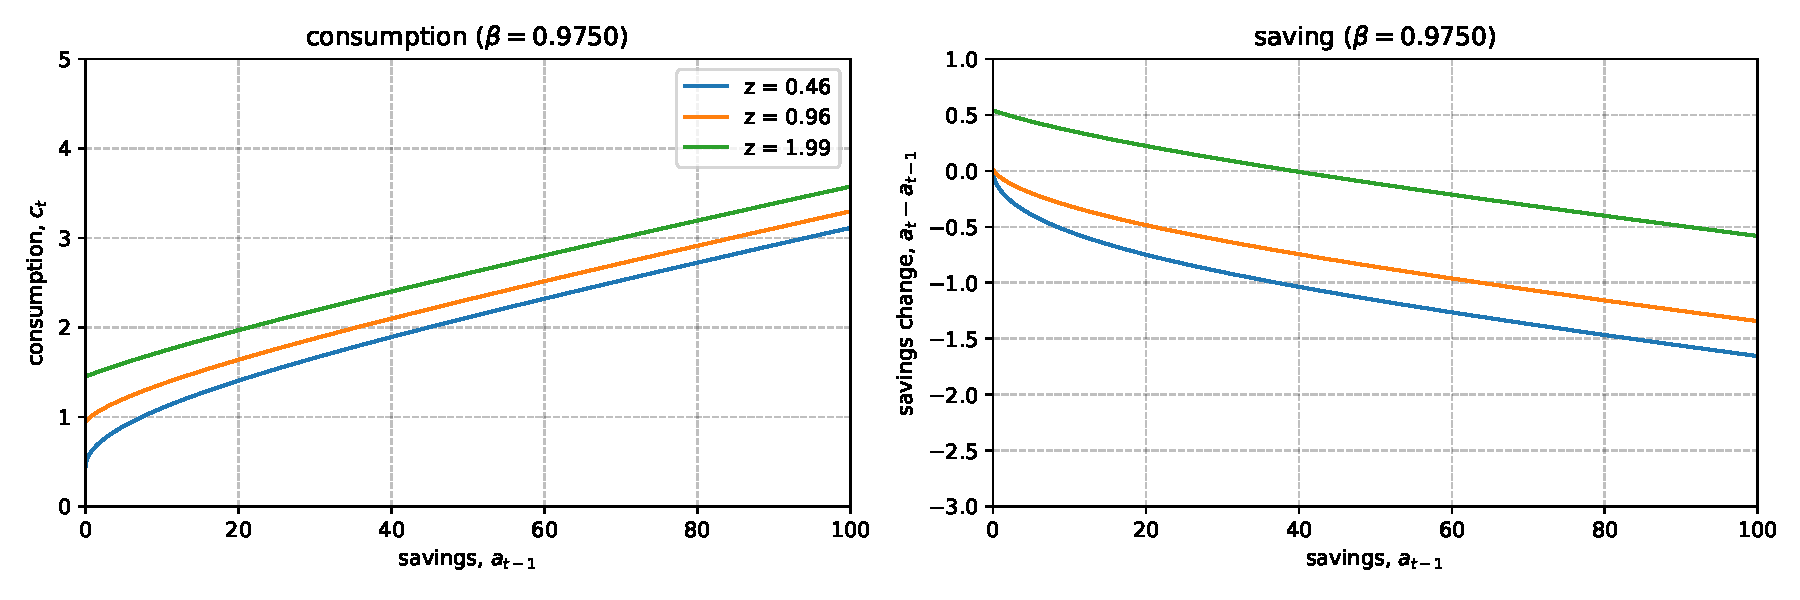
\includegraphics[width=1\textwidth]{figs/c_func_1}
\end{frame}
%
\begin{frame}{Low vs. high $\beta_{i}$}
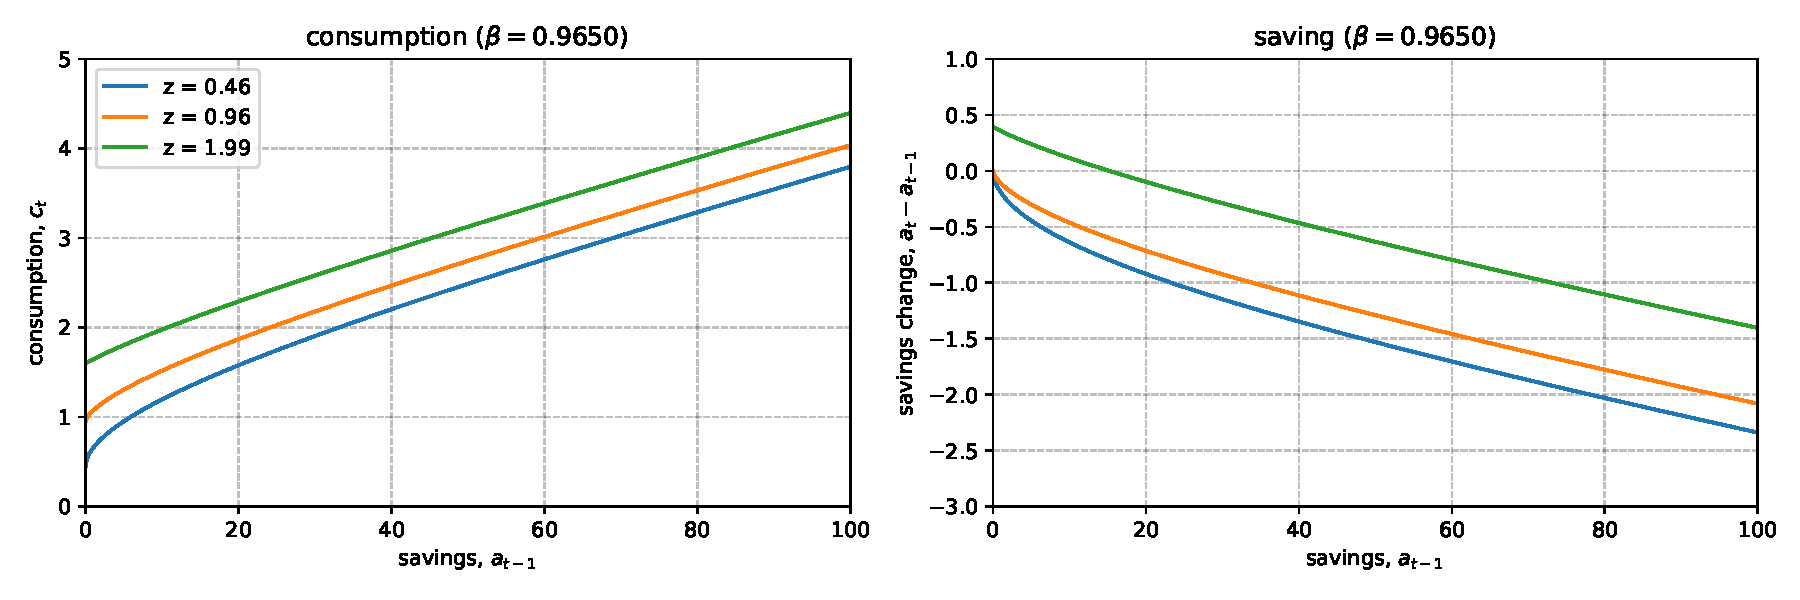
\includegraphics[width=1\textwidth]{figs/c_func_0}
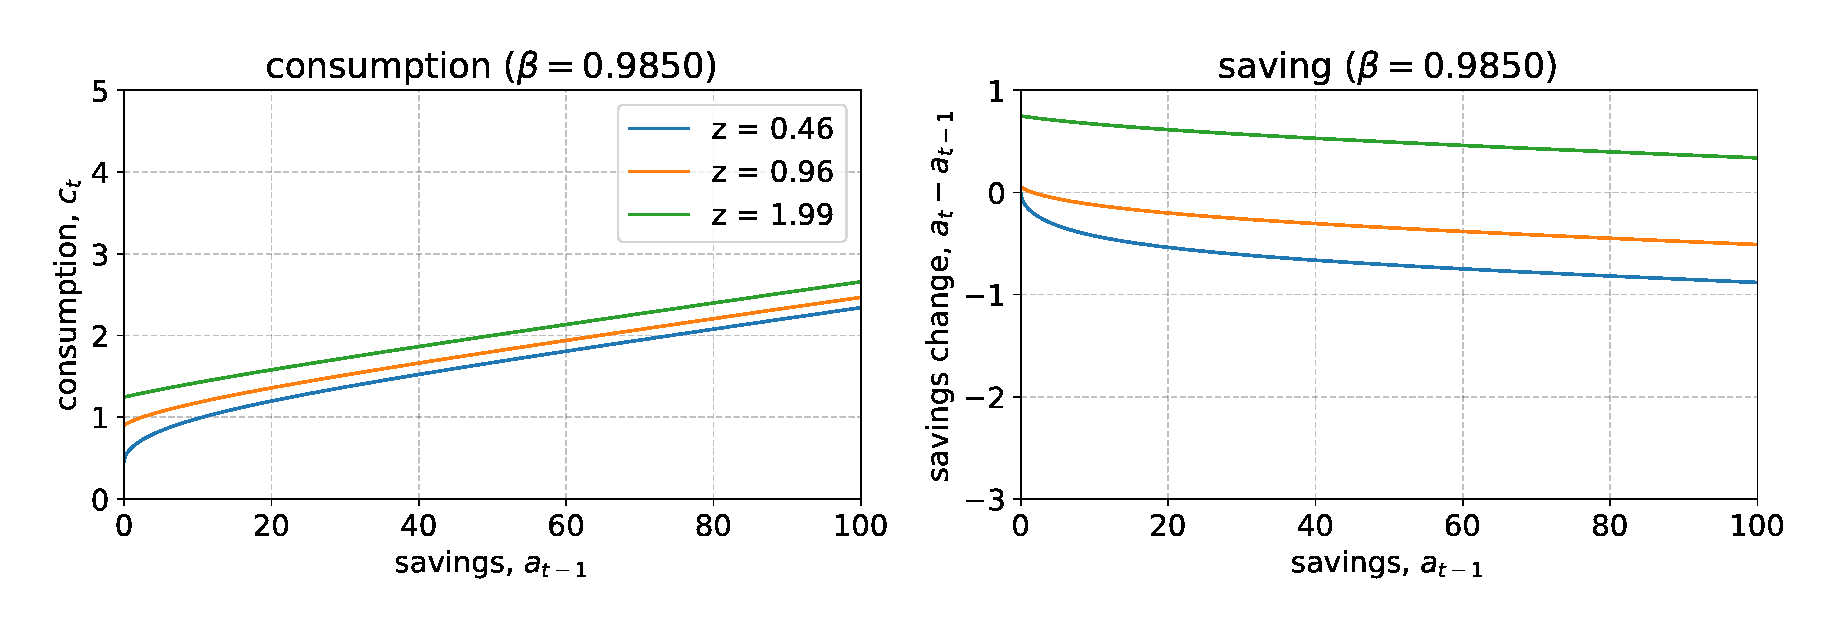
\includegraphics[width=1\textwidth]{figs/c_func_2}
\end{frame}
%
\begin{frame}{Distribution, $\boldsymbol{D}_{t}$}
\begin{itemize}
\item \textbf{Productivity: }Marginal distribution over only $z_{it}$
\item \textbf{Savings: }Marginal distribution over $a_{it}$ cond. on $\beta_{i}$
\end{itemize}
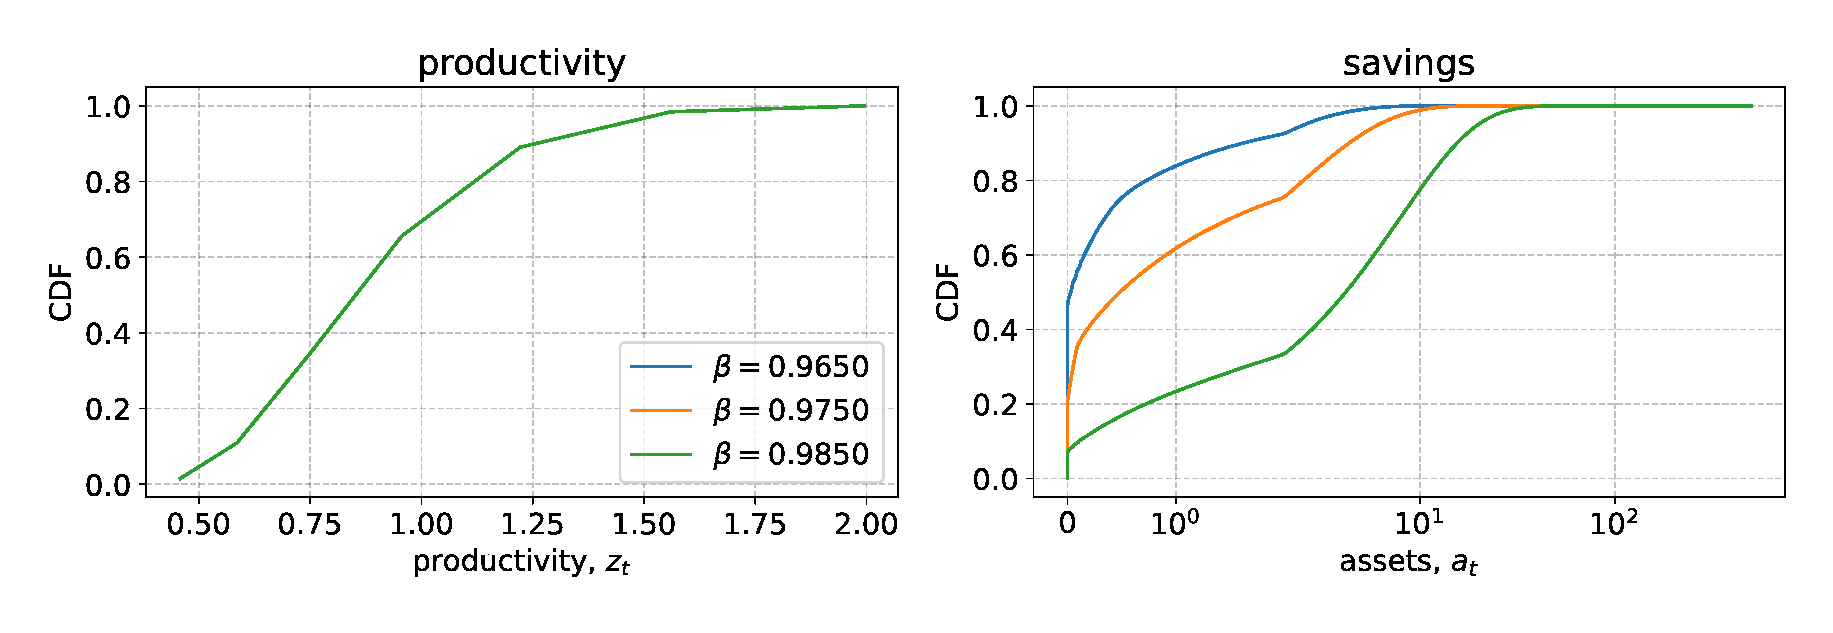
\includegraphics[width=1\textwidth]{figs/distribution}
\begin{itemize}
\item \textbf{Drivers of wealth inequality:}
\begin{enumerate}
\item Stochastic income
\item Heterogeneous patience $\rightarrow$ savings behavior
\end{enumerate}
\end{itemize}
\end{frame}
%
\begin{frame}{Steady state interest rate}
\begin{itemize}
\item <+->\textbf{Representative agent / complete markets: }
Derived from aggregate Euler-equation
\[
C_{t}^{-\sigma}=\beta(1+r_{t+1})C_{t+1}^{-\sigma}\Rightarrow C_{ss}^{-\sigma}=\beta(1+r_{ss})C_{ss}^{-\sigma}\Leftrightarrow\beta=\frac{1}{1+r_{ss}}
\]
\item <+->\textbf{Heterogeneous agents: }\emph{No such equation exists}
\begin{enumerate}
\item Euler-equation replaced by asset market clearing condition
\item Idiosyncratic income risk affects the steady state interest rate\vspace{2mm}
{\footnotesize{}}%
\begin{tabular}{|c|c|c|c|}
\hline 
{\footnotesize{}$\sigma_{\psi}$} & {\footnotesize{}PE ($r_{ss}=1\%$), $A^{hh}$} & {\footnotesize{}GE, $r_{ss}$} & {\footnotesize{}GE, $A^{hh}$}\tabularnewline
\hline 
\hline 
{\footnotesize{}$0.09$} & {\footnotesize{}$2.78$} & \textrm{\footnotesize{}$\,1.00\%$} & {\footnotesize{}$2.78$}\tabularnewline
\hline 
{\footnotesize{}$0.14$} & {\footnotesize{}$7.39$} & \textrm{\footnotesize{}~$0.12\%$} & {\footnotesize{}$2.97$}\tabularnewline
\hline 
{\footnotesize{}$0.19$} & {\footnotesize{}$13.68$} & {\footnotesize{}$-1.11\%$} & {\footnotesize{}$3.30$}\tabularnewline
\hline 
\end{tabular}\vspace{2mm}
\textbf{Partial Equilibrium}: Same interest rate.
\textbf{General Equilibrium}: Capital+labor market clearing.
\end{enumerate}
\end{itemize}
\end{frame}
%
\section{Calibration}
\begin{frame}{How to choose parameters?}
\begin{itemize}
\item <+->\textbf{External calibration: }Set subset of parameters to the
\emph{standard values in the literature} or \emph{directly from data
estimates} \\
(e.g. income process)
\item <+->\textbf{Internal calibration: }Set remaining parameters so the
model fit a number of chosen \emph{macro-level and/or micro-level}
\emph{targets }based on empirical estimates
\begin{enumerate}
\item \textbf{Informal: }Roughly match targets by hand
\item \textbf{Formal: }
2a. Solve root-finding problem
2b. Minimize a squared loss function
\item \textbf{Estimation: }Formal with squared loss function (think GMM)
or likelihood function + standard errors
\end{enumerate}
\item <+->\textbf{Complication:} \emph{We must always solve for the steady
state for each guess of the parameters to be calibrated}
\end{itemize}
\end{frame}
%
\section{Exercises}
\begin{frame}{Exercise: HANCGovModel}
\begin{itemize}
\item \textbf{No production. }No physical savings instrument
\item \textbf{Households: }Get stochastic endowment\textbf{ }$z_{it}$ of
consumption good
\item \textbf{Government:}
\begin{enumerate}
\item Choose government spending
\item Collect taxes, $\tau_{t}$, proportional to endowment
\item Bonds: Pays $1$ consumption good next period. Price is $p_{t}^{B}<1$
\begin{align*}
p_{t}^{B}B_{t} & +\int\tau_{t}z_{it}d\boldsymbol{D}_{t}=B_{t-1}+G_{t}\\
\tau_{t} & =\tau_{ss}+\eta_{t}+\varphi\left(B_{t-1}-B_{ss}\right)
\end{align*}
where $\eta_{t}$ is a tax-shifter
\end{enumerate}
\item \textbf{Market clearing:
\begin{align*}
B_{t} & =A_{t}^{hh}\\
C_{t}^{hh}+G_{t} & =\int z_{it}d\boldsymbol{D}_{t}=1
\end{align*}
}
\end{itemize}
\end{frame}
%
\begin{frame}{Exercise: Households}
\textbf{Households:}
\begin{align*}
v_{t}(z_{it},a_{it-1}) & =\max_{c_{it}}\frac{c_{it}^{1-\sigma}}{1-\sigma}+\beta\mathbb{E}_{t}\left[v_{it+1}(z_{it+1},a_{it})\right]\\
\text{s.t. }p_{t}^{B}a_{it}+c_{it} & =a_{it-1}+(1-\tau_{t})z_{it}\geq0\\
\log z_{it+1} & =\rho_{z}\log z_{it}+\psi_{it+1}\,\,\,,\psi_{it}\sim\mathcal{N}(\mu_{\psi},\sigma_{\psi}),\,\mathbb{E}[z_{it}]=1\,
\end{align*}
\textbf{Euler-equation}:
\begin{align*}
c_{it}^{-\sigma} & =\beta\frac{\underline{v}_{a,t+1}(z_{it},a_{it})}{p_{t}^{B}}
\end{align*}
\textbf{Envelope condition:
\[
\underline{v}_{a,t}(z_{it-1},a_{it-1})=c_{it}^{-\sigma}
\]
}
\end{frame}
%
\begin{frame}{Exercise: Questions}
\begin{enumerate}
\item \textbf{Define the stationary equilibrium}
\item \textbf{Solve and simulate the household problem }\\
with $p_{ss}^{B}=0.975$ and $\tau_{ss}=0.12$.
\item \textbf{Find the stationary equilibrium}\\
with $G_{ss}=0.10$ and $\tau_{ss}=0.12$.
\item \textbf{What happens for $\tau_{ss}\in(0.11,0.15)?$ }
\item \textbf{When is average household utility maximized? }
\end{enumerate}
\vspace{5mm}\textbf{Note:} Full solution in repository folder \emph{GEModelToolsNotebooks/HANCGovModel}
\end{frame}
%
\section{Summary}
\begin{frame}{Summary and next week}
\begin{itemize}
\item \textbf{Today: }
\begin{enumerate}
\item The concept of a stationary equilibrium
\item Introduction to the \textcolor{DarkRed}{\href{https://github.com/NumEconCopenhagen/GEModelTools}{GEModelTools}}
package
\end{enumerate}
\item \textbf{Next week: }\emph{Work on assignment}
\item \textbf{Exercise/Homework:}
\begin{enumerate}
\item Work on completing the HANCGovModel exercise
\item Go through \emph{Stationary-Equilibrium} notebook in repository 
\item Assignment
\end{enumerate}
\end{itemize}
\end{frame}
%
\end{document}
